\documentclass[../notes.tex]{subfiles}

\pagestyle{main}
\renewcommand{\chaptermark}[1]{\markboth{\chaptername\ \thechapter\ (#1)}{}}
\setcounter{chapter}{6}

\begin{document}




\chapter{Two-Body Systems}
\section{Two-Body Problem: Center-of-Mass Coordinates and Collisions}
\begin{itemize}
    \item \marginnote{10/30:}Announcements.
    \begin{itemize}
        \item OH regular time but in KPTC 303.
    \end{itemize}
    \item Today:
    \begin{itemize}
        \item 2 body systems, i.e., 2 bodies in a uniform force field (usually gravity).
    \end{itemize}
    \item Consider two particles with masses and positions $m_1,\vec{r}_1$ and $m_2,\vec{r}_2$ that exhibit forces on each other. We seek to describe their motion.
    \begin{itemize}
        \item To do so, we'll first develop a coordinate system in which its easy to describe their motion.
        \item Next, we'll write a Lagrangian for the system.
        \item Then, we'll use it to find equations of motion.
    \end{itemize}
    \item The first thing we'll do is develop a more convenient coordinate system than Cartesian coordinates in which to describe these two bodies.
    \begin{itemize}
        \item We'll need the sum $M$ of their masses, their center of mass $\vec{R}$, their relative position $\vec{r}$, and their reduced mass $\mu$, given as follows.
        \begin{align*}
            M &= m_1+m_2&
            \vec{R} &= \frac{m_1\vec{r}_1+m_2\vec{r}_2}{m_1+m_2}&
            \vec{r} &= \vec{r}_1-\vec{r}_2&
            \mu &= \frac{m_1m_2}{m_1+m_2} = \frac{m_1m_2}{M}
        \end{align*}
        \item In particular, $(\vec{R},\vec{r})$ are our generalized coordinates.
        \item Note: Switching to this new coordinate system is often colloquially referred to as a \textbf{diagonalization} of the system since the switch \emph{uncouples} the equations of motion of the two particles.
        \item Note: This is perhaps our first example of generalized coordinates ($\vec{R},\vec{r}$) that aren't just shifted Cartesian coordinates.
    \end{itemize}
    \item Next, we'll write the Lagrangian of the system, $L=T-V$.
    \begin{itemize}
        \item With respect to $T$, we can logically (albeit highly unintuitively) calculate that
        \begin{align*}
            T &= \frac{1}{2}m_1\dot{\vec{r}}_1^2+\frac{1}{2}m_2\dot{\vec{r}}_2^2\\
            &= \frac{1}{2}\left[ \frac{(m_1^2+m_1m_2)\dot{\vec{r}}_1^2+(m_2^2+m_1m_2)\dot{\vec{r}}_2^2}{m_1+m_2} \right]\\
            &= \frac{1}{2}\frac{(m_1\vec{r}_1+m_2\vec{r}_2)^2}{m_1+m_2}+\frac{1}{2}\frac{m_1m_2}{m_1+m_2}(\dot{\vec{r}}_1-\dot{\vec{r}}_2)^2\\
            &= \frac{1}{2}M\dot{\vec{R}}^2+\frac{1}{2}\mu\dot{\vec{r}}{\,}^2
        \end{align*}
        \item With respect to $V$, we have a uniform external force $m\vec{g}$ (e.g., $\vec{g}=-g\ihat$), so
        \begin{align*}
            V &= -m_1\vec{g}\cdot\vec{r}_1-m_2\vec{g}\cdot\vec{r}_2+V_\text{int}(\vec{r}_1-\vec{r}_2)\\
            &= -M\vec{g}\cdot\vec{R}+V_\text{int}(\vec{r})
        \end{align*}
        \item Thus, the final Lagrangian is
        \begin{equation*}
            L = \frac{1}{2}M\dot{\vec{R}}^2+M\vec{g}\cdot\vec{R}+\frac{1}{2}\mu\dot{\vec{r}}{\,}^2-V_\text{int}(\vec{r})
        \end{equation*}
    \end{itemize}
    \item What is $\mu$?
    \begin{itemize}
        \item The quantity that works. All of the above is "because it works" mathematics.
    \end{itemize}
    \item We can now find equations of motion describing the two-body system.
    \begin{itemize}
        \item Start with the E-L equations
        \begin{align*}
            \dv{t}(\pdv{L}{\dot{\vec{R}}_i}) &= \pdv{L}{\vec{R}_i}&
            \dv{t}(\pdv{L}{\dot{\vec{r}}_i}) &= \pdv{L}{\vec{r}_i}
        \end{align*}
        \item Substituting in the Lagrangian, we obtain
        \begin{align*}
            M\ddot{R}_i &= Mg_i&
            \mu\ddot{r}_i &= -\pdv{V}{r_i} = F_i(\vec{r})
        \end{align*}
        \begin{itemize}
            \item The left equation tells us that the center of mass is uniformly accelerating.
            \item The right equation is equivalent to a 1-particle problem.
        \end{itemize}
    \end{itemize}
    \item Summary of the above: The general method for solving two-body problems.
    \begin{enumerate}
        \item Solve the 1-body EOM here.
        \item Transform back to $\vec{r}_1,\vec{r}_2$ coordinates, via
        \begin{align*}
            \vec{r}_1 &= \vec{R}+\frac{m_2}{M}\vec{r}&
            \vec{r}_2 &= \vec{R}-\frac{m_1}{M}\vec{r}
        \end{align*}
    \end{enumerate}
    \item Descriptors of the system.
    \begin{itemize}
        \item When $L$ is separable, there are also 2 separately conserved energies.
        \begin{align*}
            \frac{1}{2}M\dot{\vec{R}}^2-M\vec{g}\cdot\vec{R} &= E_\text{cm}&
            \frac{1}{2}\mu\dot{\vec{r}}{\,}^2+V_\text{int}(\vec{r}) &= E_\text{int}
        \end{align*}
        \item The total linear momentum of the system.
        \begin{equation*}
            \vec{P} = m\dot{\vec{r}}_1+m_2\dot{\vec{r}}_2 = M\vec{R}
        \end{equation*}
        \item The total angular momentum of the system.
        \begin{align*}
            \vec{J} &= m_1\vec{r}_1\times\dot{\vec{r}}_1+m_2\vec{r}_2\times\dot{\vec{r}}_2\\
            &= m_1\left( \vec{R}+\frac{m_2}{M}\vec{r} \right)\times\left( \dot{\vec{R}}+\frac{m_2}{M}\dot{\vec{r}} \right)+m_2\left( \vec{R}-\frac{m_1}{M}\vec{r} \right)\times\left( \dot{\vec{R}}-\frac{m_1}{M}\dot{\vec{R}} \right)\\
            &= M\vec{R}\times\dot{\vec{R}}+\mu\vec{r}\times\dot{\vec{r}}
        \end{align*}
    \end{itemize}
    \item The center of mass frame.
    \begin{itemize}
        \item Vectors in this frame are denoted with a superscript $*$.
        \item In the center of mass frame, we define $\vec{R}^*=0$. That is, we let the origin of our coordinate system lie at the center of mass and move with it.
        \item We now explore some characteristics of this frame.
        \item It follows from this choice and the aforementioned coordinate transformations that
        \begin{align*}
            \vec{r}_1{}^* &= \frac{m_2}{M}\vec{r}&
            \vec{r}_2{}^* &= -\frac{m_1}{M}\vec{r}
        \end{align*}
        \item Additionally, the momenta of the two particle are equal and opposite:
        \begin{equation*}
            m_1{\dot{\vec{r}}_1}^* = -m_2{\dot{\vec{r}}_2}^* = \mu\dot{\vec{r}} = \vec{p}{\,}^*
        \end{equation*}
        \item It follows from the above that if the velocity of the center of mass is $\dot{\vec{R}}$, then we have
        \begin{align*}
            \vec{p}_1 &= m_1\dot{\vec{r}}_1 = m_1\dot{\vec{R}}+\vec{p}{\,}^*&
            \vec{p}_2 &= m_2\dot{\vec{r}}_2 = m_2\dot{\vec{R}}-\vec{p}{\,}^*
        \end{align*}
        \item The total momentum, angular momentum, and kinetic energy in the CM frame are
        \begin{align*}
            \vec{P}^* &= 0&
            \vec{J}^* &= \mu\vec{r}\times\dot{\vec{r}} = \vec{r}\times\vec{p}{\,}^*&
            T^* &= \frac{1}{2}\mu\dot{\vec{r}}{\,}^2 = \frac{(\vec{p}{\,}^*)^2}{2\mu}
        \end{align*}
        \item Once again, converting these values back to another frame in which the velocity of the center of mass is $\dot{\vec{R}}$, we obtain
        \begin{align*}
            \vec{P} &= M\dot{\vec{R}}&
            \vec{J} &= M\vec{R}\times\dot{\vec{R}}+\vec{J}^*&
            T &= \frac{1}{2}M\dot{\vec{R}}^2+T^*
        \end{align*}
    \end{itemize}
    \item Example: Large satellite (e.g., moon around earth).
    \begin{figure}[h!]
        \centering
        \begin{tikzpicture}
            \footnotesize
            \draw [densely dashed] circle (3mm);
            \draw [densely dashed] circle (1cm);
    
            \fill [blx] (-110:0.3) circle (2.5pt);
            \fill [gray] (70:1) circle (1.5pt);
    
            \fill circle (1pt) node[fill=white,right=1pt]{CM};
            \draw [<-,thick] (110:1) -- (109:1);
            \draw [<-,thick] ({110+180}:0.3) -- ({109+180}:0.3);
        \end{tikzpicture}
        \caption{Moon and Earth in CM frame.}
        \label{fig:CMmoonEarth}
    \end{figure}
    \begin{itemize}
        \item Physically, the two tethered celestial bodies both orbit their center of mass.
        \item However, mathematically, this is equivalent to a particle of mass $\mu$ orbiting a fixed point mass $M$. Indeed, the EOM for $\vec{r}$ is
        \begin{equation*}
            \mu\ddot{\vec{r}} = -\hat{r}\frac{Gm_1m_2}{r^2}
            = -\hat{r}\frac{GM\mu}{r^2}
        \end{equation*}
        \item Thus, the period of the (assumed) elliptical orbit can be calculated using the same methods as before. Indeed, we obtain
        \begin{equation*}
            \left( \frac{\tau}{2\pi} \right) = \frac{a^3}{GM}
        \end{equation*}
        \begin{itemize}
            \item However, note that $a$ is the semimajor axis of the \emph{relative} orbit (i.e., is the median distance between the bodies) and that $M$ is the \emph{sum} of the masses rather than the mass of the heavier body.
            \item Takeaway: Kepler's third law is only \emph{approximately} correct.
        \end{itemize}
        \item To conclude, let's discuss the motion of the Earth and moon in the CM frame.
        \begin{itemize}
            \item Herein, the Earth orbits the CM with a small radius, and the moon orbits the CM directly across from the Earth in a much larger orbit.
            \item Mathematically,
            \begin{align*}
                \vec{r}_1{}^* &= \frac{m_2}{M}\vec{r}&
                \vec{r}_2{}^* &= -\frac{m_1}{M}\vec{r}
            \end{align*}
            where we approximate
            \begin{align*}
                \frac{m_2}{M} &\approx \frac{1}{82}&
                \frac{m_1}{M} &\approx \frac{81}{82}
            \end{align*}
        \end{itemize}
    \end{itemize}
    \item We now switch to an important application of this CM theory.
    \item \textbf{Elastic} (collision): A collision between two particles in which the kinetic energy is the same before and after.
    \begin{figure}[h!]
        \centering
        \begin{subfigure}[b]{0.35\linewidth}
            \centering
            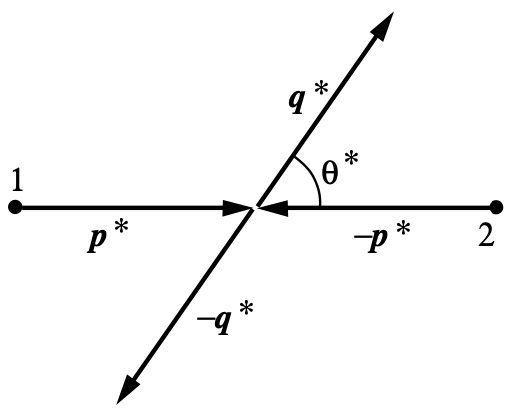
\includegraphics[width=0.8\linewidth]{../ExtFiles/CMelastica.png}
            \caption{CM frame.}
            \label{fig:CMelastica}
        \end{subfigure}
        \begin{subfigure}[b]{0.35\linewidth}
            \centering
            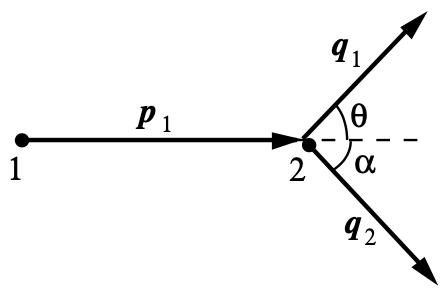
\includegraphics[width=0.7\linewidth]{../ExtFiles/CMelasticb.png}
            \caption{Lab frame.}
            \label{fig:CMelasticb}
        \end{subfigure}\\[1em]
        \begin{subfigure}[b]{0.35\linewidth}
            \centering
            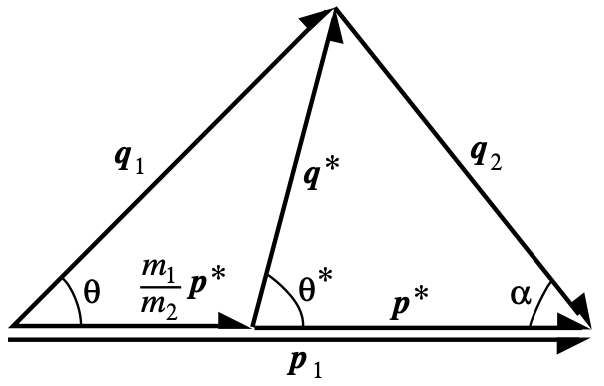
\includegraphics[width=0.9\linewidth]{../ExtFiles/CMelasticc.png}
            \caption{Relations.}
            \label{fig:CMelasticc}
        \end{subfigure}
        \begin{subfigure}[b]{0.35\linewidth}
            \centering
            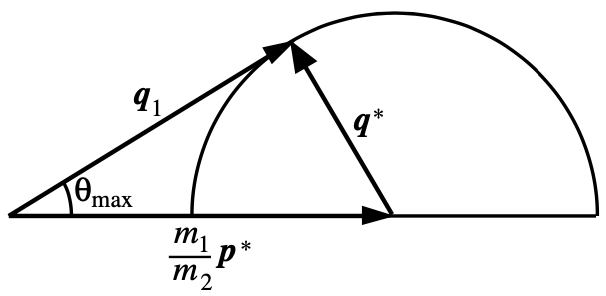
\includegraphics[width=0.95\linewidth]{../ExtFiles/CMelasticd.png}
            \caption{$\theta_\text{max}$.}
            \label{fig:CMelasticd}
        \end{subfigure}
        \caption{Elastic collisions.}
        \label{fig:CMelastic}
    \end{figure}
    \begin{itemize}
        \item Examples: Hard spheres, Coulomb force, gravity.
        \item Takeaways from Figure \ref{fig:CMelastica}.
        \begin{itemize}
            \item Here's what an elastic collision looks like in the CM frame: We have two particles coming in, one with momentum $\vec{p}{\,}^*$ and one with momentum $-\vec{p}{\,}^*$. After the collision, the particles separate with momenta $\vec{q}{\,}^*$ and $-\vec{q}{\,}^*$.
            \item Since energy is conserved,
            \begin{equation*}
                T^* = \frac{(\vec{p}{\,}^*)^2}{2m} = \frac{(\vec{q}{\,}^*)^2}{2m}
            \end{equation*}
            \item Thus, the magnitudes of the momenta before and after the collision are the same, i.e.,
            \begin{equation*}
                p^* = q^*
            \end{equation*}
        \end{itemize}
        \item Takeaways from Figure \ref{fig:CMelasticb}.
        \begin{itemize}
            \item In the lab, most elastic collision experiments begin with one incoming particle and one particle at rest.
            \item Denote by $\vec{p}_1$ the lab momentum of the incoming particle and by $\vec{p}_2$ the lab momentum of the resting particle. Note that
            \begin{align*}
                \vec{p}_1 &= m_1\dot{\vec{R}}+\vec{p}{\,}^*&
                \vec{p}_2 &= m_2\dot{\vec{R}}-\vec{p}{\,}^*
            \end{align*}
            \item Now observe that $\vec{p}_2=0$. Then it follows from the right equation above that
            \begin{equation*}
                \dot{\vec{R}} = \frac{1}{m_2}\vec{p}{\,}^*
            \end{equation*}
            \item Substituting this into the left equation above yields
            \begin{equation*}
                \vec{p}_1 = \frac{m_1}{m_2}\vec{p}{\,}^*+\vec{p}{\,}^* = \frac{M}{m_2}\vec{p}{\,}^*
            \end{equation*}
            \item Therefore, employing the equations that shift you out of the CM frame and the above, we obtain
            \begin{align*}
                \vec{q}_1 &= m_1\dot{\vec{R}}+\vec{q}{\,}^*&
                    \vec{q}_2 &= m_2\dot{\vec{R}}-\vec{q}{\,}^*\\
                &= \frac{m_1}{m_2}\vec{p}{\,}^*+\vec{q}{\,}^*&
                    &= \vec{p}{\,}^*-\vec{q}{\,}^*
            \end{align*}
        \end{itemize}
        \item Question to address: How much kinetic energy can be transferred during a collision?
        \begin{itemize}
            \item The lab kinetic energy transferred to the target particle is
            \begin{equation*}
                T_2 = \frac{q_2^2}{2m_2}
            \end{equation*}
            \item From Figure \ref{fig:CMelasticc}, we have that
            \begin{align*}
                \alpha &= \frac{1}{2}(\pi-\theta^*)&
                q_2 &= 2p^*\sin\frac{1}{2}\theta^*
            \end{align*}
            \item Combining these two results into the $T_2$ formula yields
            \begin{align*}
                T_2 &= \frac{2(p^*)^2}{m_2}\sin^2\frac{1}{2}\theta^*\\
                \frac{T_2}{T} &= \frac{\frac{2(p^*)^2}{m_2}\sin^2\frac{1}{2}\theta^*}{\frac{p_1^2}{2m_1}}\\
                &= \frac{\frac{2(p^*)^2}{m_2}\sin^2\frac{1}{2}\theta^*}{\frac{M^2(p_1^*)^2}{2m_1m_2^2}}\\
                &= \frac{4m_1m_2}{M^2}\sin^2\frac{1}{2}\theta^*
            \end{align*}
            \item The maximum occurs when $\theta^*=\pi$ and has value
            \begin{equation*}
                \frac{T_2}{T} = \frac{4m_1m_2}{M^2}
            \end{equation*}
            \item Note that the expression on the right, above, equals unity when $m_1=m_2$.
        \end{itemize}
        \item Relating the lab and CM scattering angles.
        \begin{equation*}
            \tan\theta = \frac{\sin\theta^*}{m_1/m_2+\cos\theta^*}
        \end{equation*}
        \begin{itemize}
            \item We read the above from Figure \ref{fig:CMelasticc} by dropping a perpendicular from the upper vertex.
            \item If $m_1=m_2$:
            \begin{align*}
                \theta &= \frac{\theta^*}{2}&
                \theta_\text{max} &= \frac{\pi}{2}
            \end{align*}
            \item If $m_1/m_2>1$:
            \begin{equation*}
                \sin\theta_\text{max} = \frac{m_2}{m_1}
            \end{equation*}
            \item Example: An $\alpha$ particle can only be scattered by a proton by up to \ang{14.5}, and a proton can only be scattered by an electron by up to \ang{0.031}.
            \item Note that $\theta_\text{max}$ can be visualized as in Figure \ref{fig:CMelasticd}.
        \end{itemize}
    \end{itemize}
\end{itemize}



\section{Office Hours (Jerison)}
\begin{itemize}
    \item What is the differential scattering cross-section, intuitively?
    \begin{itemize}
        \item It's weird notation, because it's really a function of the scattering angle $\Theta$.
        \item It's the rate of particles exiting at angle $\Theta$ per unit solid angle.
        \begin{itemize}
            \item So as we increase the area on the surface of the scatterer that we're considering (i.e., increase $\dd{\Omega}$), the flux of particles bouncing off of the sphere (i.e., rate of particles exiting at angle $\Theta$) increases a certain amount, which varies depending on characteristics of the system.
        \end{itemize}
        \item It depends on $b,\sin\theta,\dv*{b}{\theta}$, where $b(\Theta)$ depends on the particular force law or potential.
        \item We can derive $b(\Theta)$ from constraints of the system.
        \begin{itemize}
            \item The general formula from the homework is relevant!
        \end{itemize}
        \item Then $\dv*{\sigma}{\Omega}$ can tell us things about our system.
        \item Reread Sections 4.5 and 4.7 of \textcite{bib:KibbleBerkshire} in depth!
    \end{itemize}
    \item What are Lagrange undetermined multipliers?
    \begin{itemize}
        \item Jerison gives the definition.
    \end{itemize}
    \item Lagrange undetermined multipliers with multiple constraints?
    \begin{itemize}
        \item Jerison goes through the Atwood Machine --- Example 7.8 from \textcite{bib:ThorntonMarion}.
    \end{itemize}
    \item How do we convert between the following two expressions?
    \begin{align*}
        x(t) &= A\cos(\omega t)+B\sin(\omega t)&
        x(t) &= a\cos(\omega t-\theta)
    \end{align*}
    \begin{itemize}
        \item Use the trig identity $\cos(x-y)=\cos(x)\cos(y)+\sin(x)\sin(y)$.
        \item Thus,
        \begin{equation*}
            x(t) = a[\cos(\omega t)\cos\theta+\sin(\omega t)\sin\theta]
        \end{equation*}
        \item It follows that we can identify $A=a\cos\theta$ and $B=a\sin\theta$.
    \end{itemize}
    \item Some thoughts on circular orbits.
    \item Fundamental constants.
    \begin{itemize}
        \item Formulas will not be provided, but any fundamental constants (e.g., radius of earth or gravitational constant $G$) will be provided.
        \item No calculators for the exam! They are not needed. If you don't want to work out the numerical value for something, leaving an expression is fine.
        \item Exam is designed to be easier and faster than the PSets.
        \item The most complicated things will not appear.
        \item Driven oscillators are fair game, but nothing horribly complicated will be there.
        \item No Greens functions or general periodic forcing (Fourier analysis) will appear.
    \end{itemize}
    \item You, the textbook, and the pset answer key have, at times, referred to equations of constraint as "Euler-Lagrange equations" in the context of the method of Lagrange undetermined multipliers. Why?
    \item Why doesn't my solution to the bead on a rotating wire work with the method of Lagrange's undetermined multipliers?
    \begin{itemize}
        \item Proper approach.
        \begin{itemize}
            \item Use 3 equations ($y,r,\theta$) and 2 constraints ($\theta=\omega t$,$z=cr^2$) to find 5 variables $y,r,\theta,\lambda_1,\lambda_2$.
            \item We do not use $r=R$ until the end because this is not \emph{technically} a force of constraint. Indeed, the particle is still free to move along the wire here, i.e., there is no reason we could not take the system and then push the bead down with our finger, while there is a reason we could not slow the wire or push it off the parabola with our finger.
        \end{itemize}
        \item Thus, the solution works out something like this.
        \begin{itemize}
            \item The Lagrangian is
            \begin{equation*}
                L = \frac{1}{2}m(\dot{r}^2+r^2\dot{\theta}^2+\dot{z}^2)-mgz
            \end{equation*}
            \item Lagrange's 5 equations are
            \begin{align*}
                mr\dot{\theta}^2-m\ddot{r}-2cr\lambda_1 &= 0\\
                -2mr\dot{r}\theta-mr^2\dot{\theta}+\lambda_2 &= 0\\
                -mg-m\ddot{z}+\lambda_1 &= 0\\
                z-cr^2 &= 0\\
                \theta-\omega t &= 0
            \end{align*}
            \item After inserting $r=R$ and its consequence $\dot{r}=\ddot{r}=\dot{z}=\ddot{z}=0$, these simplify quite a bit to
            \begin{align*}
                m\dot{\theta}^2-2c\lambda_1 &= 0\\
                -mR^2\dot{\theta}+\lambda_2 &= 0\\
                -mg+\lambda_1 &= 0\\
                z-cR^2 &= 0\\
                \theta-\omega t &= 0
            \end{align*}
            \item Substituting $\lambda_1=mg$ and $\dot{\theta}=\omega$ into the first line above and simplifying yields the desired result.
            \begin{align*}
                m\omega^2-2cmg &= 0\\
                \omega^2-2cg &= 0\\
                c &= \frac{\omega^2}{2g}
            \end{align*}
        \end{itemize}
    \end{itemize}
\end{itemize}



\section{Chapter 7: The Two-Body Problem}
\emph{From \textcite{bib:KibbleBerkshire}.}
\begin{itemize}
    \item \marginnote{10/31:}Focus: Isolated system of two particles with an internal force.
    \item We will also touch on the presence of a uniform gravitational field, as that does not make the problem any more difficult to solve.
    \item Consider two particles of masses $m_1,m_2$ at positions $\vec{r}_1,\vec{r}_2$.
    \item Let $\vec{F}:=\vec{F}_{12}$.
    \item EOMs of the two particles in a uniform gravitational field.
    \begin{align*}
        m_1\ddot{\vec{r}}_1 &= m_1\vec{g}+\vec{F}&
        m_2\ddot{\vec{r}}_2 &= m_2\vec{g}-\vec{F}
    \end{align*}
    \item \textbf{Center of mass}: The point defined as follows for two particles of masses $m_1,m_2$ at positions $\vec{r}_1,\vec{r}_2$. \emph{Denoted by} $\bm{\vec{R}}$, $\bm{\vec{\bar{r}}}$. \emph{Given by}
    \begin{equation*}
        \vec{R} = \frac{m_1\vec{r}_1+m_2\vec{r}_2}{m_1+m_2}
    \end{equation*}
    \item Definition of \textbf{relative position} (see Chapter 1).
    \item The vectors and scalars describing a two body system may be visualized as follows.
    \begin{figure}[h!]
        \centering
        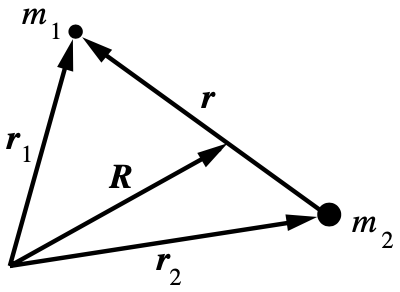
\includegraphics[width=0.2\linewidth]{../ExtFiles/2BodySystem.png}
        \caption{Two-body system.}
        \label{fig:2BodySystem}
    \end{figure}
    \item \textbf{Reduced mass}: The quantity defined as follows. \emph{Denoted by} $\bm{\mu}$. \emph{Given by}
    \begin{equation*}
        \mu = \frac{m_1m_2}{m_1+m_2}
    \end{equation*}
    \begin{itemize}
        \item The reduced mass is named as such "because it is always less than either $m_1$ or $m_2$" \parencite[160]{bib:KibbleBerkshire}.
    \end{itemize}
    \item From the EOMs above, we can derive (as in class) that
    \begin{align*}
        M\ddot{\vec{R}} &= M\vec{g}&
        \mu\ddot{\vec{r}} &= \vec{F}
    \end{align*}
    \item General procedure and conservation laws.
    \item Lagrangian approach.
    \item \textbf{Center-of-mass frame}: Teh frame of reference in which the center of mass is at rest at the origin. \emph{Also known as} \textbf{CM frame}.
    \item Another section that we did not cover in class: CM and Lab Cross-Sections.
\end{itemize}




\end{document}